\documentclass[a4paper, 12pt]{article}%тип документа

%отступы
\usepackage[left=2cm,right=2cm,top=2cm,bottom=3cm,bindingoffset=0cm]{geometry}

%Русский язык
\usepackage[T2A]{fontenc} %кодировка
\usepackage[utf8]{inputenc} %кодировка исходного кода
\usepackage[english,russian]{babel} %локализация и переносы

%Вставка картинок
\usepackage{wrapfig}
\usepackage{graphicx}
\graphicspath{{pictures/}}
\DeclareGraphicsExtensions{.pdf,.png,.jpg}

%оглавление
\usepackage{titlesec}
\titlespacing{\chapter}{0pt}{-30pt}{12pt}
\titlespacing{\section}{\parindent}{5mm}{5mm}
\titlespacing{\subsection}{\parindent}{5mm}{5mm}
\usepackage{setspace}

%Графики
\usepackage{multirow}
\usepackage{pgfplots}
\pgfplotsset{compat=1.9}

%Математика
\usepackage{amsmath, amsfonts, amssymb, amsthm, mathtools}

%Заголовок
\author{Валеев Рауф Раушанович \\
группа 825}
\title{\textbf{Работа 3.4.5\\
Петля гистерезиса (динамический метод)}}
\newtheorem{task}{Задача}
\begin{document}
\maketitle
\newpage
\section*{Цель работы}
Исследование предельных петель гистерезиса и начальных кривых намагничивания для нескольких ферромагнитных образцов; определение магнитных характеристик материалов, чувствительность каналов $X$ и $Y$ осциллографа и постоянную времени $\tau$ интегрирующей цепочки.
\section*{В работе используются}
автотрансформатор, понижающий трансформатор, амперметр и вольтметр, резистор, делитель напряжения, интегрирующая цепочка, электронный осциллограф, тороидальные образцы с двумя обмотками.
\section*{Экспериментальная установка}
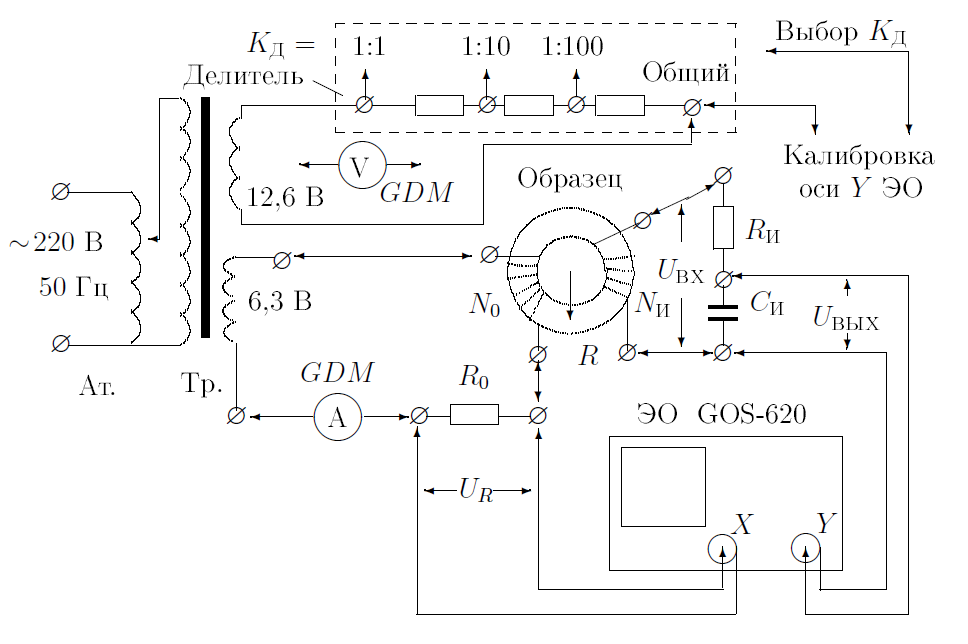
\includegraphics[width = \textwidth]{1.png}

Действующее значение переменного тока в обмотке $N_0$ измеряется амперметром $A$. Последовательно с амперметром включено сопротивление $R_0$, напряжение с которого подается на вход $X$ электронного осциллографа. Это напряжение пропорционально току в обмотке $N_0$, а следовательно и напряженности $H$ магнитного поля в образце.

Для измерения магнитной индукции $B$ с измерительной обмотки $N_{\text{и}}$ на вход интегрирующей $RC$-цепочки подается напряжение $U_{\text{и}}(U_{\text{вх}})$, пропорциональное $\dot{B}$, а, с выхода снимается напряжение $U_{\text{с}}(U_{\text{вых}})$, пропорциональное величине $B$, а подается на вход $Y$.

\section*{Теория}
\subsection*{Измерение напряжения с помощью осциллографа}
Исследуемый сигнал подается на вход $X$; длина $2x$ горизонтальной черты, наблюдаемой на экране, характеризует удвоенную амплитуду сигнала. 

Если известна чувствительность усилителя $K_x$ в вольтах на деление шкалы экрана, то удвоенная амплитуда напряжения определяется произведением
\[2U_{X, 0} = 2x \cdot K_x\]
Напряжение, подаваемое на вход $Y$ определяется аналогично. 

Калибровку осей осциллографа можно использовать для построения кривой гистерезиса в координатах $B$ и $H$:

Зная величину сопротивления $R_0$, с которого снимается сигнал, можно определить чувствительность канала по току $K_{XI} = \dfrac{K_x}{R_0}$ [A/дел]; затем, используя формулу 
\begin{equation}
H = \dfrac{IN_0}{2\pi R}
\end{equation}
определить цену деления шкалы в A/м.

Используя формулу 
\begin{equation}
B = \dfrac{R_{\text{и}}C_{\text{и}}U_{\text{вых}}}{SN_{\text{и}}}
\end{equation}
можно рассчитать цену деления вертикальной шкалы в теслах.
\subsection*{Проверка калибровки горизонтальной оси ЭО с помощью амперметра}
проводится при закороченной обмотке $N_0$. Эта обмотка с помещенным в нее ферромагнитным образцом является нелинейным элементом, так что ток в ней не имеет синусоидальной формы, и это не позволяет связать амплитуду тока с показаниями амперметра.
\begin{equation}
m_X = \dfrac{2 \sqrt{2} R_0 I_{\text{эф}}}{2x} \text{[B/дел]}
\end{equation}
\subsection*{Проверка калибровки вертикальной оси ЭО с помощью вольтметра}
Сигнал с обмотки 12,6 В понижающего трансформатора подается на делитель напряжения. Часть этого напряжения снимается с делителя с коэффициентом деления $K_{\text{Д}}$ (1/10 или 1/100) и подается на вход $Y$. Мультиметр $V$ измеряет напряжение $U_{\text{эф}}$ на этих же клеммах делителя.

Далее по формуле 
\begin{equation}
m_Y = \dfrac{2\sqrt{2}U_{\text{эф}}}{2y} \text{[B/дел]}
\end{equation}
можно рассчитать чувствительность канала $Y$.
\subsection*{Постоянная времени $RC$-цепочки}
Рассчитывается по формуле 
\begin{equation}
RC = \dfrac{U_{\text{вх}}}{\Omega U_{\text{вых}}}
\end{equation}
\section*{Ход работы}
\subsection*{Петля гистерезиса}
Запишем некоторые характеристики образцов в таблицу
\begin{center}
\begin{tabular}{|c|c|c|c|}
\hline
 & Пермаллой & Кремнистое железо & Феррит 1000нн \\ \hline
$N_0$ & 15 & 20 & 45 \\ \hline
$N_{\text{и}}$ & 300 & 200 & 400 \\ \hline
$S$, см$^2$ & 0,66 & 2 & 3 \\ \hline
$2\pi R$, см & 14,1 & 11 & 25 \\ \hline
\end{tabular}\\
\textbf{Таблица 1.} Некоторые характеристики образцов.
\end{center}
\begin{center}
\begin{tabular}{|c|c|}
\hline
$R_0$, Ом & 0,2 \\ \hline
$R_{\text{и}}$, кОм & 20 \\ \hline
$C_{\text{и}}$, мкФ & 20 \\ \hline
\end{tabular}\\
\textbf{Таблица 2.} Некоторые параметры установки.
\end{center}
Далее получим предельную петлю, нанесем ее на кальку и снимем на нее же начальную кривую намагничивания, постепенно уменьшая ток.

Восстановим предельную петлю, измерим двойные амплитуды для коэрцитивной силы $[2x(c)]$ и индукции насыщения $[2y(s)]$. Запишем амплитуды и $K_X$, $K_Y$ в таблицу. По формулам $(1)$ и $(2)$, подставив $I = K_X/R_0$, $U_{\text{вых}} = K_Y$. Получив цену деления мы можем посчитать $H_c$ и $B_s$.

Повторим эти действия для всех образцов и занесем их в таблицу.
\begin{center}
\begin{tabular}{|c|c|c|c|c|c|c|}
\hline
 & Величина & $\sigma$ & Величина & $\sigma$ & Величина & $\sigma$ \\ \hline
 & \multicolumn{2}{c|}{Пермаллой} & \multicolumn{2}{c|}{Феррит 1000нн} & \multicolumn{2}{c|}{Кремнистое железо} \\ \hline
Петля & \multicolumn{2}{c|}{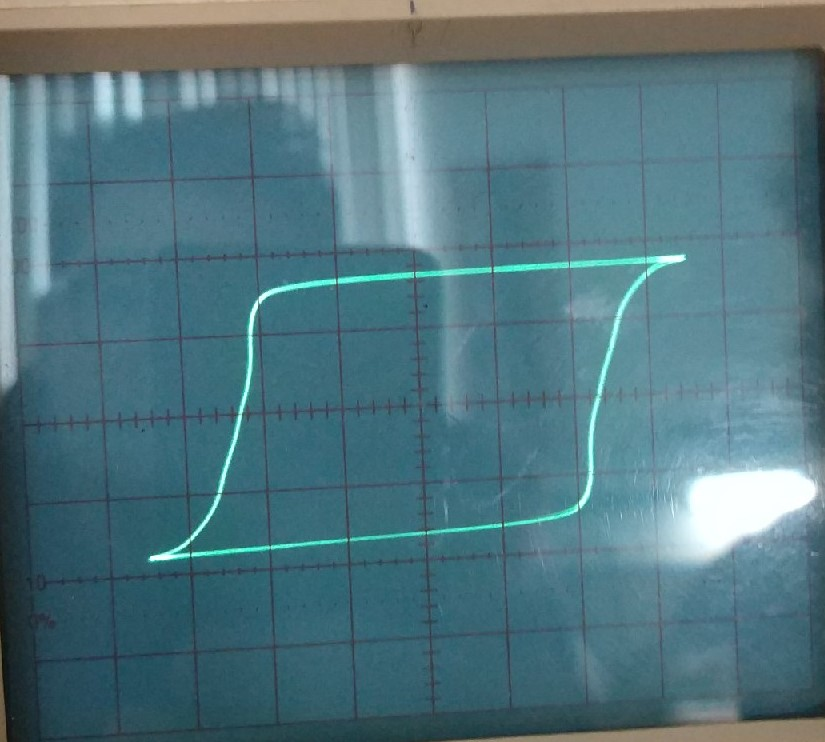
\includegraphics[width = 0.2\textwidth]{2.jpg}} &  \multicolumn{2}{c|}{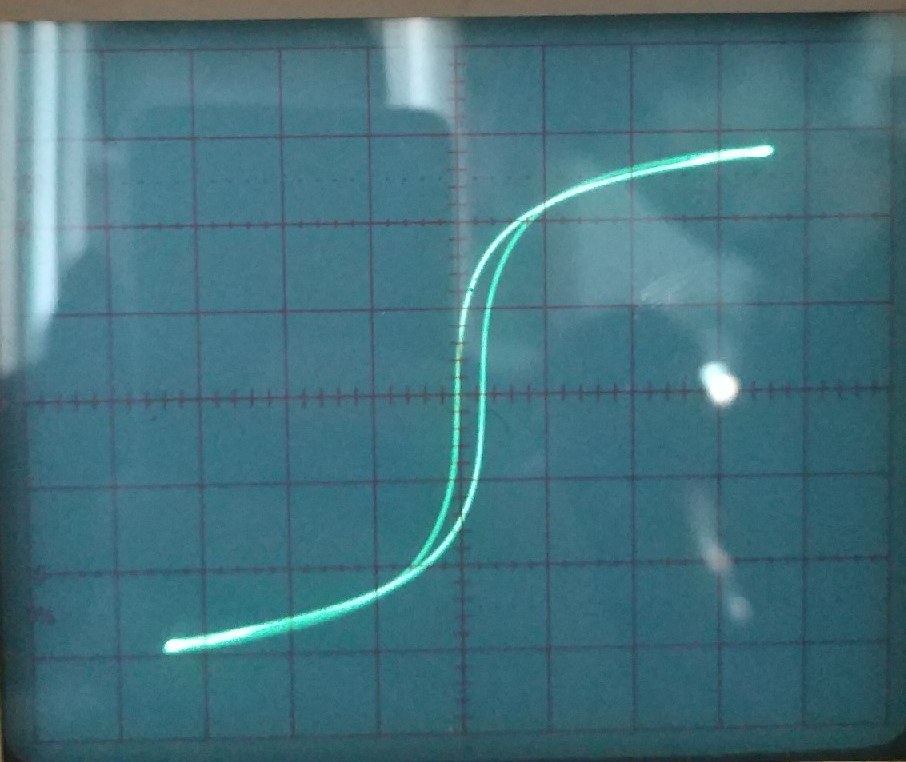
\includegraphics[width = 0.2\textwidth]{3.jpg}} &  \multicolumn{2}{c|}{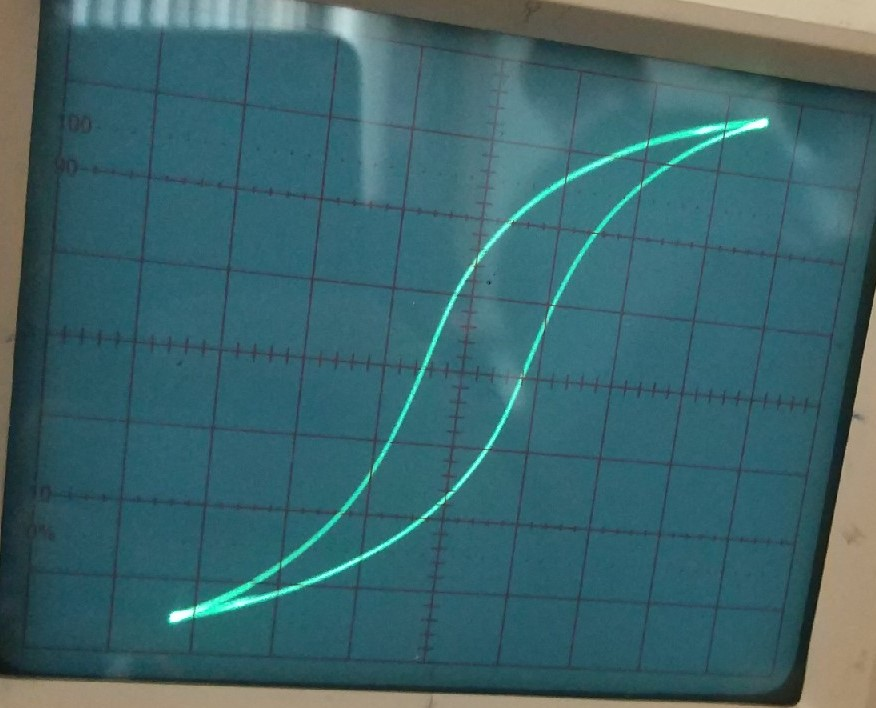
\includegraphics[width = 0.2\textwidth]{4.jpg}} \\ \hline
$I_{\text{эф}}$, А & 0,217 & 0,001 & 0,570 & 0,001 & 1,000 & 0,001 \\ \hline
$[2x(c)]$, ед & 4,4 & 0,2 & 7,0 & 0,2 & 7,0 & 0,2 \\ \hline
$[2y(s)]$, ед & 3,2 & 0,2 & 6,0 & 0,2 & 5,8 & 0,2 \\ \hline
$K_x$ & 0,02 & 0 & 0,02 & 0 & 0,05 & 0 \\ \hline
$K_y$ & 0,05 & 0 & 0,1 & 0 & 0,02 & 0 \\ \hline
$H$, А/м & 10,6 & 0,02 & 18,2 & 0,2 & 45 & 0,3 \\ \hline
$H_c$, А/м & 47 & 6 & 132 & 11 & 320 & 20 \\ \hline
$B$, Тл/дел & 1,012 & 0,011 & 1,000 & 0,011 & 0,067 & 0,002 \\ \hline
$B_s$, Тл & 3,2 & 0,2 & 6,0 & 0,2 & 0,39 & 0,02 \\ \hline
\end{tabular}\\
\textbf{Таблица 3.} Данные, полученные из петли гистерезиса.
\end{center}
\subsection*{Проверка калибровки оси $X$}
Отключаем намагничивающую обмотку от цепи, соединив оба провода, идущих к обмотке, на одной из ее клемм. 

Подбираем такой ток, чтобы горизонтальная прямая занимала большую часть экрана.

Рассчитаем чувствительность канала $m_X$ по формуле $(3)$. 

Результаты смотри в таблице 3.
\subsection*{Проверка калибровки оси $Y$}
Разберем цепь. Соединим вход $Y$ с клеммами делителя "1/100-земля". Не меняя рабочего коэффициента $K_Y$, подберем с помощью трансформатора напряжение, при котором вертикальная прямая занимает почти весь экран. Измеряем длину $2y$. Запишем данные из двух вышеизложенных пунктов в таблицу. Рассчитаем $m_Y$ по формуле $(4)$.

\begin{center}
\begin{tabular}{|c|c|c|c|c|c|c|}
\hline
 & Величина & $\sigma$ & Величина & $\sigma$ & Величина & $\sigma$ \\ \hline
 & \multicolumn{2}{c|}{Пермаллой} & \multicolumn{2}{c|}{Феррит 1000нн} & \multicolumn{2}{c|}{Кремнистое железо} \\ \hline
$2x$, ед & 6,0 & 0,1 & 7,0 & 0,1 & 10,0 & 0,1 \\ \hline
$m_X$, {[}B/дел{]} & 0,020 & 0,001 & 0,092 & 0,001 & 0,057 & 0,001 \\ \hline
$U_{\text{эф}}$, В & 0,13 & 0,01 & 0,50 & 0,01 & 0,50 & 0,01 \\ \hline
$2y$, ед & 8,0 & 0,1 & 7,0 & 0,1 & 7,0 & 0,1 \\ \hline
$m_Y$, {[}B/дел{]} & 0,046 & 0,001 & 0,202 & 0,001 & 0,202 & 0,001 \\ \hline
$K_x$ & 0,02 & 0 & 0,02 & 0 & 0,05 & 0 \\ \hline
$K_y$ & 0,05 & 0 & 0,1 & 0 & 0,02 & 0 \\ \hline
\end{tabular}\\
\textbf{Таблица 4.} Калибровка осей осциллографа.
\end{center}
По таблице видим, что соответствующие $K$ и $m$ равны с точностью то погрешности.
\section*{Расчет $\tau$ постоянной времени для цепочки}
Считаем $U_{\text{вх}} = 2y \cdot K_y$ и $U_{\text{вых}} = 2x \cdot K_x$.

Запишем все полученные данные в таблицу и посчитаем $\tau$ по формуле $(5)$ и через параметры установки.
\begin{center}
\begin{tabular}{|c|c|c|}
\hline
Величина & Значение & Ошибка \\ \hline
$2y$, ед & 8,0 & 0,2 \\ \hline
$K_y$, В/ед & 2 & 0 \\ \hline
$2x$, ед & 6,2 & 0,2 \\ \hline
$K_x$, В/ед & 0,02 & 0 \\ \hline
$U_{\text{вх}}$, В & 16,0 & 0,2 \\ \hline
$U_{\text{вых}}$, В & 0,124 & 0,002 \\ \hline
$\tau$ из формулы, c & 0,41 & 0,02 \\ \hline
$\tau$ из пар. уст., c & 0,40 & 0,02 \\ \hline
\end{tabular}\\
\textbf{Таблица 5.} Измерение $\tau$.
\end{center}
\newpage
Сравним $H_c$ и $B_s$ с табличными.
\begin{center}
\begin{tabular}{|c|c|c|c|c|}
\hline
 & Ампл. & Fe-Ni & Fe-Si & Феррит \\ \hline
эксп & \multirow{2}{*}{$H_c$, A/м} & $47 \pm 6$ & $320 \pm 20$ & $132 \pm 11$ \\ \cline{1-1} \cline{3-5} 
табл &  & 4 & 8 & 8-600 \\ \hline
эксп & \multirow{2}{*}{$B_s$, Тл} & $3,2 \pm 0,2$ & $0,39 \pm 0,02$ & $6,0 \pm 0,2$ \\ \cline{1-1} \cline{3-5} 
табл &  & 1,08 & 2 & 0,2-0,4 \\ \hline
\end{tabular}\\
\textbf{Таблица 6.} Сверка с табличными значениями.
\end{center}

\section*{Литература}
\begin{enumerate}
\item \textbf{Лабораторный практикум по общей физике:} Учебное пособие. В трех томах. Т. 2. Электричество и магнетизм /Гладун А.Д., Александров Д.А., Берулёва Н.С. и др.; Под ред. А.Д. Гладуна - М.: МФТИ, 2007. - 280 с.
\item \textbf{Дополнительное описание лабораторной работы 3.3.5}: Эффект Холла в металлах; Под ред. МФТИ, 2016. - 5 с.
\end{enumerate}
\end{document}

